\input{wg21common}

% Footnotes at bottom of page:
 \usepackage[bottom]{footmisc} 

% Table going across a page: 
 \usepackage{longtable}

 % Start sections at 0
% \setcounter{section}{-1}

\begin{document}
\title{Contracts for C++: Revisiting contract check elision and duplication}
\author{ Timur Doumler \small(\href{mailto:papers@timur.audio}{papers@timur.audio}) 
}
\date{}
\maketitle

\begin{tabular}{ll}
Document \#: & D3228R1 \\
Date: &2024-04-20 \\
Project: & Programming Language C++ \\
Audience: & SG21, EWG
\end{tabular}

\begin{abstract}
This paper attempts to inform and structure to the discussion whether the Contracts MVP should retain the rule that checked contract assertions are allowed to be evaluated any number of times when checking a contract predicate, or tighten it to require exactly one evaluation, or possibly some interval of allowed values. We list the different conflicting design requirements and the possible specification solutions, and provide an analysis of which solutions satisfy which design requirements.
\end{abstract}

%%%%%%%%%%%%%%%%%%%%%%%%%%%%%%%%%%%%%%%%%%%%%

\section{Introduction}
\label{sec:intro}

The current Contracts MVP \cite{P2900R6}, as forwarded by SG21 to EWG and LEWG for design review, allows contract predicates that have side effects when evaluated. While side effects that modify the essential behaviour of the program are discouraged (contract assertions should assert the correctness of a program without altering it), other side effects can be useful. For example, when performing a contract check, the user might want to do things like allocating memory (for example, to perform an algorithm that asserts some non-trivial property of a range), lock and unlock a mutex (for example, to assert the value of a variable that can be accessed concurrently), or maintain some state (for example, to assert that the depth of a recursive function call or the number of times a particular statement has been executed has not exceeded a certain limit). Even \cite{P2680R1}, a direction paper proposing that contract predicates with side effects should be ill-formed by default, allowed for ``relaxed'' predicates that can exhibit such side effects. We therefore need to have a solid specification for how such predicates should behave.

\cite{P2900R6} currently specifies that for a \emph{checked} contract assertion, the predicate evaluation may be elided if the compiler can prove that the result of such an evaluation would be \tcode{true} or \tcode{false}. Further, it specifies that at any point within a contract assertion sequence, any previously evaluated contract assertions may be evaluated again, and such repetitions can occur an arbitrary number of times. Effectively this means that, if a predicate has observable side effects, those side effects may occur zero, one or more times, with no upper bound on the number of possible evaluations.

At the March 2024 WG21 meeting in Tokyo, several issues with this approach were discovered, leading to the realisation that SG21 needs to rediscuss this part of \cite{P2900R6}'s specification and either adopt a different solution that addresses these issues, or at least reconfirm that we consider the current design correct and strengthen the motivation for it.  This paper serves to inform and structure that discussion.

%%%%%%%%%%%%%%%%%%%%%%%%%%%%%%%%%%%%%%%%%%%%%

\section{History and context}

In C++2a Contracts \cite{P0542R5}, as adopted into the C++20 Working Draft, the issue of contract check elision and duplication did not arise, because evaluating a contract predicate that has observable side effects was specified to be undefined behaviour, and for contract predicates without side effects, elision and duplication is unobservable under the as-if rule.

The paper \cite{P1670R0} proposed to change C++2a Contracts to make predicates with side effects well-defined but allow elision of the predicate evaluation. This paper was never adopted into the C++20 Working Draft because Contracts were removed from it before the paper was considered, however it made its way into an early version of the Contracts MVP \cite{P2388R4}, which additionally allowed to \emph{duplicate} the evaluation. This went through several iterations. \cite{P2388R0} allowed to elide or duplicate all (as opposed to ``some') side effects of the evaluated predicate, as long as this does not affect the result of that evaluation. \cite{P2388R3} relaxed this to allow eliding or duplicating such side effects per subexpression of a predicate. \cite{P2521R5} strengthened it again to ``all side effects''.

As work on the Contracts MVP progressed, SG21 spent an extensive amount of time discussing this topic. \cite{P2751R1} proposed to loosen the \cite{P2521R5} model: instead of just allowing elision or duplication, the number of evaluations of a \emph{checked} contract assertion is deliberately made \emph{unspecified}. Such an evaluation can therefore be elided, evaluated once, twice, or even more times, with no specified upper bound. A counter-proposal, \cite{P2756R0}, instead proposed to strengthen the \cite{P2521R5} model by specifying that the predicate of a checked contract should be evaluated exactly once. SG21 ended up adopting  \cite{P2751R1} and rejecting \cite{P2756R0} (poll results see \cite{P2751R1}, Section 5).

Independently from the discussion around these papers, the direction paper \cite{P2680R1} proposed a design direction whereby contract predicates with side effects would be ill-formed by default. However, even this paper provided an escape hatch in the form of so-called ``relaxed'' predicates that can exhibit side effects, and therefore did not remove the need to specify the behaviour of such predicates (an issue that the paper itself did not address). The design direction proposed by \cite{P2680R1} ultimately failed to get consensus in SG21.

At the March 2024 WG21 meeting in Tokyo, \cite{P2900R6}  went through a first round of design review in EWG. This design review has revealed several issues with the current approach:
\begin{itemize}
\item A contract assertion that will exhibit undefined behaviour after a number of repeated assertions (say, repeated signed integer addition) can be considered to exhibit undefined behaviour always, as there is no specified upper bound on the number of evaluations;
\item Low-latency and real-time systems require a deterministic upper bound on the runtime complexity of a contract assertion;
\item For some safety-critical systems, a deterministic upper bound is not sufficient, and a guarantee is required that a checked assertion is evaluated a known, deterministic number of times.
\end{itemize} 

In addition, an EWG guidance poll revealed that a significant number of people prefer that contract assertions should not be allowed to be evaluated more than once (poll results see \cite{D3197R0}, Poll 7).  

The paper \cite{P3119R0} was written in response to EWG's review. It attempts to address the issues with undefined behaviour and the lack of a deterministic upper bound by introducing an implementation-defined upper bound, and recommending a value of 64. However, the paper does not attempt to address requests by EWG members that the number of evaluations be specified as exactly once or not more than once. Given that the room is currently split on this issue, the solution proposed in \cite{P3119R0} may be insufficient and we may have to at least consider a stronger model if we wish to gain approval by EWG, CWG, and Plenary for adding a Contracts MVP to C++26. The roadmap paper \cite{D3197R0} therefore proposes to rediscuss this issue in SG21.

%%%%%%%%%%%%%%%%%%%%%%%%%%%%%%%%%%%%%%%%%%%%%

\section{Scope of this paper}

This paper does not propose any concrete changes to the Contracts MVP. Instead, it lists the different conflicting design requirements and the possible specification solutions, and provides an analysis of which solutions satisfy which design requirements. The intent of the paper is to add some structure to the discussion and to highlight the engineering tradeoffs that each solution involves, to help SG21 reach consensus.

We do not consider \emph{unchecked} contract assertions (those having the \emph{ignore} evaluation semantic), as such evaluations do not involve evaluating the predicate.

Further, we do not consider contract predicates that have no observable side effects. Under the as-if rule, it is unobservable whether such ``pure'' predicates are evaluated zero, one, or multiple times, as long as the compiler has correctly determined whether the result of such an evaluation would be \tcode{true} or \tcode{false}. We therefore only consider contract predicates that have \emph{observable side effects} when evaluated. 

Finally, we do not consider contract assertions whose evaluation may end up being elided because of undefined behaviour occurring either during evaluation of the predicate itself or elsewhere in the program. We only consider programs that would have well-defined behaviour when the predicate is evaluated once.


%%%%%%%%%%%%%%%%%%%%%%%%%%%%%%%%%%%%%%%%%%%%%

\section{Design requirements}
\label{sec:reqs}

In this section, we summarise the different, partially conflicting design requirements that have motivated different proposals in this space.

\subsection{Deterministic number of evaluations}
\label{subsec:determ}
There are several reasons why a guarantee that the predicate is evaluated a deterministic number of times may be desirable.

More generally, a deterministic number of evaluations is required if we wish to minimise the amount of implementation-defined and unspecified behaviour added to the C++ language by the Contracts MVP. This is something that has been brought up as a significant concern in EWG.

More specifically, deterministic behaviour is a requirement in some safety-critical systems, which may be unable to use Contracts at all unless this requirement is satisfied. Note that this does not necessarily mean a deterministic execution time, or a deterministic sequence of CPU instructions, but a deterministic observable behaviour with regard to side effects. In other words, eliding the evaluation of a side-effect-free predicate would be a normal optimisation transformation and unobservable under the as-if rule, while eliding the evaluation of a predicate with side effects would make the behaviour of a \emph{checked} contract assertion observably non-deterministic, which is undesirable. The only situation where this happens in the language today is copy elision; some consider it undesirable to add more such situations.

Contract predicates that neither maintain internal state nor modify the state of the program still can have observable side effects. Examples that occur in practice are checking a value in the contract predicate that may be concurrently accessed from other threads, which requires locking a mutex and unlocking it again afterwards, or allocating a scratch buffer for an algorithm that proves some property on a range passed into or returned from a function. It might be beneficial to be able to reason about how many times such a contract assertion will attempt to acquire a lock, or allocate memory, rather than having such events occur an unspecified, non-deterministic amount of times when contract checks are enabled.

\subsection{Exactly one evaluation}
If we constrain ``deterministic number of evaluations'' further to ``exactly one evaluation'', we gain more potentially desirable properties. ``Exactly one evaluation'' seems to be the only reasonable implementation of ``deterministic number of evaluations'' (we see no possible reason why one would want to specify, for example, that each contract assertion is always evaluated twice), therefore we consider them to be the same requirement for the remainder of this paper.

\cite{P2756R0} argues that ``exactly one evaluation'' is the most simple, intuitive, and easy to reason about solution, and the only one that follows existing practice in \tcode{assert} and similar macros. This is also the approach that all other programming languages with a Contracts facility (Ada, D\footnote{Notably, the D programming language actually has a facility to reject functions with side effects at compile time --- functions can be annotated to be ``pure'' --- but chooses to not require contract predicates to be ``pure''. Contract predicates are therefore allowed to have side effects, like in the other programming languages, which are guaranteed to occur either zero times (when contract checks are off) or exactly once (when contract checks are on), although the D documentation does note that predicates with side effects are discouraged.}, Eiffel, etc.) follow: contract checks can be enabled or disabled, but when they are enabled, the predicate is evaluated exactly once, and any potential side effects are observed exactly once. It is therefore likely that this is the behaviour most users would assume when they start using the new C++ Contracts facility.

Assertions that rely on being evaluated exactly once when checking is enabled are common in practice. For example, one might want to add an assertion counting the number of times a recursion or iteration occurs, or the number of times a certain statement is executed, and report a contract violation if this number exceeds some fixed limit. Consider the following example (adapted from Clang):
\begin{codeblock}
#ifndef NDEBUG
  unsigned nIter = 0;
#endif
  while (item->isVariant()) {
    assert(++nIter < 6 && "Variants are nested deeper than the supported limit");
    // ...
  }
\end{codeblock}
Without a guarantee that the predicate is evaluated exactly once when the assertion is checked, this code would break, as the assertion could end up failing when it should pass, or passing when it should fail, potentially leading to undefined behaviour. Note that the above contract assertion is maintaining state and has a side effect when evaluated, but that is contained to the assertion itself and does not modify the state of the program or any other assertions.

The assertion as written above would not work with the current Contracts MVP because \cite{P2900R6} does not offer a facility like \tcode{NDEBUG} for conditionally declaring a variable only when the associated contract assertion is checked. Further, in \cite{P2900R6}, local variables such as \tcode{nIter} are implicitly const and would need to be wrapped into a \tcode{const_cast} in order to be incremented in the contract predicate. However, even without any of these limitations, any predicate that maintains and updates state like the one above cannot ever be made to work if there is no guarantee that \emph{checked} contract predicates are evaluated exactly once. 

Such predicates exist and are relatively common in existing code bases, as can be easily verified by a code search\footnote{\url{https://codesearch.isocpp.org/cgi-bin/cgi_ppsearch?q=assert\%28\%2B\%2B&search=Search}}. Further, it is possible that there are cases where such a predicate, when used with \tcode{assert}, does not wrap the declaration of the counter in an \tcode{\#ifdef NDEBUG} block, and the counter is not a local variable, but one with static or thread-local storage duration, meaning that changing such an \tcode{assert} to a \tcode{contract_assert} would silently break the program and potentially introduce undefined behaviour, without any compiler warning or other message to the user.

\cite{P2900R6} argues that such predicates should not exist, as they modify the state of the program they are supposed to merely observe, violating the design principles that the Contracts MVP is based on. We can also argue that the Contracts MVP is deliberately not designed to serve as a drop-in replacement for \tcode{assert} and should not be used in that way. This is all well and good, but in practice users will likely use the Contracts MVP in that way anyway: they are used to ``exactly one evaluation when checked'' from existing assertion macros and will intuitively expect the same behaviour. The possibility of silent code breakage and introduction of undefined behaviour by turning deterministic into non-deterministic evaluation is arguably a particularly user-hostile way to break these users' assumptions, and could significantly hamper the adoption of Contracts.

\subsection{Deterministic upper bound on number of evaluations}
\label{subsec:upper}

Many low-latency and real-time systems do not necessarily require full deterministic behaviour, but do require a deterministic upper bound on the runtime complexity of a contract assertion. These systems may be unable to use Contracts at all unless this requirement is satisfied.

In addition, without such a deterministic upper bound, a contract assertion that will exhibit undefined behaviour after a number of repeated assertions (say, repeated, accumulating signed integer addition) can be considered to exhibit undefined behaviour always; a particularly hostile compiler may treat such contract assertions as unreachable code while being conforming. Both of these issues are discussed in more detail in \cite{P3119R0}.

There are two ways to specify such an upper bound: either normatively specify a concrete number in the Standard (for example, ``at most two evaluations''), or merely specify that an implementation has to define \emph{some} deterministic upper bound but leave the actual number unspecified. The latter is proposed by \cite{P3119R0}. For consumer-facing real-time applications like video games and audio processing software which often need to support different compilers, a normatively specified upper bound seems preferable to an implementation-defined one, because the latter could change across compilers or even across different versions of the same compiler, making it harder to reason about the code and the guarantees it provides. In addition, it is unclear to what degree either option is acceptable instead of the stricter ``deterministic number of evaluations'' guarantee for such applications; this will most likely depend on the concrete use case.

\subsection{Allow duplications}
\label{subsec:ville}

The main motivation for allowing duplication of predicate evaluations is to allow the implementation to perform both caller- and callee-side checking while preserving ABI compatibility.

Note that only a subset of contract checks can be implemented caller-side\footnote{Note that, if we adopt the proposed design in \cite{P3097R0} and \cite{P3165R0} for supporting function contract assertions on virtual functions, the reverse will also become true: only a subset of contract checks can be implemented callee-side. In particular, checks for function contract assertions of the statically called function in a virtual function call can only be generated caller-side as the statically called function is unknown to the callee.}. Some contract checks must be performed callee-side, for example, when a function is called indirectly, such as through a function pointer or a facility like \tcode{std::function}\footnote{In such scenarios, a callee-side check can be generated only if the compiler front-end sees the function contract assertion related to the function call, i.e. it knows which function will be called and can see the declaration of that function.}, or when checking postconditions in the Microsoft ABI, as this ABI performs argument destruction callee-side and postcondition checks are guaranteed to happen before argument destruction. 

Now, consider a shared library that has function contract assertions on its function declarations, and an application that uses this library by compiling against a static library header and then dynamically loading a compiled library binary. The developer of the application needs to have the choice of compiling the application with caller-checks either disabled or enabled (the latter resulting in the caller-checkable subset of the library checks being checked, which can be useful to diagnose problems). Likewise, the provider of the shared library needs the choice to ship the compiled library binary with callee-side checks disabled or enabled (the latter being a ``hardened'' version of the library). Either version of the application should be able to use either version of the library binary without having to recompile and re-link\footnote{Without this requirement, guaranteeing that contract checks be evaluated exactly once would be relatively easy: If in the library, checks are disabled, in the application we call a thunk wrapper, which checks precondition assertions and then calls the function; otherwise, we just call the function. The library's build never affects whether the preconditions are checked, only the application build does. However, in this implementation model, we cannot flip precondition checks on and off by just building the library differently and then running an unmodified application with it; instead, we would need to recompile the application, which might be prohibitively slow or impossible.}. The combination of the application having caller-side checks enabled and the library having callee-side checks enabled will result in some library checks being checked twice. 

We can consider implementation strategies that would allow this use case while also guaranteeing that contract checks be evaluated exactly once (or not more than once), but such strategies come with tradeoffs. One possible strategy would be to compile the library binary such that each function with precondition or postcondition assertions has two entry points, one that performs the callee-side check and one that does not. However, this can significantly increase the amount of symbols in the binary, and requires a change to the ABI. Another possibility is to compile the library such that the choice whether to perform callee-side checks is made dynamically, but this incurs additional runtime overhead and again requires a change to the ABI.

For some users, the tradeoffs of either strategy will be unacceptable: a global ABI break might make this approach undeployable, and in a world where some C++ applications require tens of gigabytes of memory to link due to the sheer amount of symbols, there is a strong incentive to avoid adding more symbols. Further, there is currently no implementation experience for either strategy\footnote{Caller-side checking itself does not have implementation experience either, but it is arguably somewhat less theoretical, because compilers know how to parse the function contract specifiers of a function declaration and rewrite a function call \tcode{f()} into a caller-side checked function call such as \mbox{\tcode{(pre_check() ? f() : abort())}}.}. Avoiding such tradeoffs however requires us to either explicitly allow duplication of predicate evaluations, or to place this use case outside of the scope of the C++ Standard and treat support for it as a non-conforming vendor extension, as we do for example for \tcode{-fno-exceptions}.

\cite{P2751R1} discusses other reasons why allowing duplication would be beneficial.

\subsection{Allow elisions}
\label{subsec:elisions}

One might want to allow eliding contract predicates along with their observable side effects, in a fashion similar to copy elision, if the compiler can prove that the result of the elided evaluation would be \tcode{true} or \tcode{false}. For example, if a function \tcode{f} has a checked precondition assertion \tcode{pre(x)}, and immediately after that, as the first statement in the body of \tcode{f}, another function \tcode{g} with a functionally equivalent precondition assertion is called, eliding the latter assertion would avoid unnecessarily evaluating the expression \tcode{x} twice. This is discussed in more detail in \cite{P2751R1}.

\subsection{Allow more than two repetitions}
\label{subsec:rep}

While supporting both caller- and callee-side checking in the same program without an ABI break or extra symbols may require allowing evaluation to occur twice, we are not aware of any scenario where evaluation could end up occurring three times or more. It seems therefore that it would be enough to allow evaluation to occur up to twice, rather than an unspecified number of times. However, \cite{P3119R0} describes a use case for which allowing an unspecified number larger than 2 might be useful. A user might want to test for destructive contract assertions (contract assertions with undesirable side effects) by evaluating them repeatedly during testing and observing if results change.  Such tests are a good way to gain confidence that the contract predicates are not doing something that fundamentally breaks the program's behaviour: destructive effects are more likely to be noticeable when evaluating the predicate, say, 16 times, than when evaluating it twice. By allowing more than two repetitions, the specification would allow a compiler to provide a conforming option to request an arbitrary number of repetitions for performing such tests.

\subsection{Make the number of evaluations unspecified}
\label{subsec:discourage}

One might want to make the number of evaluations deliberately unspecified to further discourage users from writing predicates with side effects as they learn that they cannot rely on the behaviour of such predicates: the side effects may occur any number of times or not at all. This is discussed in more detail in \cite{P1670R0} and \cite{P2751R1}.

Not relying on side effects in contract predicates is stated as an important design principle in \cite{P2900R6}. The philosophy is that contract assertions should be able to test the correctness of the programs that did not yet have those assertions in them, which effectively means that they need to test the correctness of the same program when those assertions are ignored and not some other program. If, however, the predicates alter the behaviour such that the new, altered program is then correct (or incorrect), such contract assertions fail at diagnosing any defects and instead themselves introduce Heisenbugs. Note that assertions with side effects are nevertheless found in real-world code bases, and can be useful, such as the counter described in Section~\ref{subsec:determ}.

\subsection{Avoid numbers other than 0, 1, ``many''}
\label{subsec:01many}

Another possible reason to prefer an unspecified number of evaluations instead of ``up to 2'' is the wish to avoid magic numbers like 2 in the specification of the C++ Standard, and stick to the options 0, 1, or ``many'' that are preferred in some computer science contexts.

%%%%%%%%%%%%%%%%%%%%%%%%%%%%%%%%%%%%%%%%%%%%%

\section{The solution space}
\label{sec:prepost}

We begin by listing all plausible specification strategies for how many times the predicate of a checked contract assertion may be evaluated. Whether elisions are allowed is orthogonal to the other concerns, so we can split the solution space into solutions that allow elisions and solutions that do not. The four known solutions that allow elisions are as follows (all four have been proposed somewhere at some point):
\renewcommand{\theenumi}{$\Alph{enumi}_0$} \begin{enumerate}
\item At most once, i.e. evaluation may be elided but not duplicated (\cite{P1670R0}, \cite{D3197R0} poll 7).
\item At most twice (\cite{P2521R5}), i.e. evaluation may be both elided and duplicated.
\item An unspecified number of times, with an implementation-defined upper bound $N$ (\cite{P3119R0} proposal 3).
\item An unspecified number of times, with no upper bound (status quo, \cite{P2900R6}).
\end{enumerate}
Further, we can construct four solutions that are analogous to the above but do not allow elisions (only one of those, $A_1$, has been formally proposed):
\renewcommand{\theenumi}{$\Alph{enumi}_1$} \begin{enumerate}
\item Exactly once (\cite{P2756R0}).
\item Once or twice, i.e. evaluation may be duplicated but not elided.
\item An unspecified number of times, with an implementation-defined upper bound $N$, but at least once.
\item An unspecified number of times, with no upper bound, but at least once.
\end{enumerate}

 Remember that we only consider evaluations of contract assertions with \emph{checked} evaluation semantics (\tcode{observe}, \tcode{enforce}, or \tcode{quick_enforce}), as evaluations with \emph{unchecked} evaluation semantics (\tcode{ignore}) always evaluate the predicate zero times and we do not consider removing \tcode{ignore} from the MVP or changing how it is specified. Remember further that we only consider evaluation of predicates with observable side effects. For predicates with no observable side effects, neither elision nor duplication are observable under the as-if rule, and therefore all of the above solutions are equivalent. 

A few more solutions than the ones listed above are theoretically possible, such as requiring a deterministic number of evaluations that is not once (e.g. ``every contract assertion must always be evaluated twice''), or requiring a normatively specified (as opposed to implementation-defined) upper bound larger than two. We do not consider these solutions here because we are not aware of any benefits these might have over the ones listed above. 

Further, there has been a suggestion that we could allow duplications and simultaneously ensure a deterministic amount of evaluations with a solution that says that the predicate must be evaluated exactly $N$ times, where $N$ is implementation-defined. An implementation may then say that, for example, $N$ is 1 if the function called is in a statically linked library, but 2 if the library is linked dynamically. However, a conforming implementation may satisfy such a specification by simply saying that $N$ is any number between 0 and 64 (for example), therefore such a solution is equivalent to solution $C_0$.

%%%%%%%%%%%%%%%%%%%%%%%%%%%%%%%%%%%%%%%%%%%%%

\section{Choosing the best solution}
\subsection{\tcode{pre} and \tcode{post}}
Now that we enumerated both the requirements and the possible solutions, we can create a decision matrix listing which possible solutions satisfy which design requirements. The decision matrix for \tcode{pre} and \tcode{post} is given in Table~\ref{table:matrix}.


%%%%%%%%%%%%%%%%%%%%%%%%%%%%%%%%%%%%%%%%%%%%%
%\vspace{4mm}
\begin{table}%[!htbp]
\begin{tabular}{|p{5.4cm}|p{0.9cm}|p{0.9cm}|p{0.9cm}|p{0.9cm}|p{0.9cm}|p{0.9cm}|p{0.9cm}|p{0.9cm}|}
\hline 
Design requirement & $A_0$ & $A_1$ & $B_0$ & $B_1$ & $C_0$ & $C_1$ & $D_0$ & $D_1$ \\
\phantom{xxxxxxxxxxxi}Nr. of evaluations:& 0 -- 1 & 1 & 0 -- 2& 1 -- 2 & 0 -- $N$ & 1 -- $N$ & \mbox{0 -- $\infty$} & \mbox{1 -- $\infty$} \\
\hline
1. Normatively specify a deterministic number of evaluations / exactly one evaluation& no & yes & no & no & no & no & no & no \\
\hline
2. Normatively specify a concrete, deterministic upper bound on number of evaluations & yes & yes & yes & yes & no & no & no & no \\
\hline
3. Require \emph{some} deterministic upper bound on number of evaluations & yes & yes & yes & yes & yes & yes & no & no \\
\hline
4. Allow duplication of evaluations to facilitate caller-/callee-side checking compatibility & no & no & yes & yes  & yes & yes & yes & yes \\
\hline
5. Allow elision of evaluations if compiler can prove predicate would evaluate to \tcode{true} or \tcode{false} & yes & no & yes & no & yes & no & yes & no \\
\hline
6. Allow more than two repetitions to test for destructive contract assertions & no & no & no & no & yes & yes & yes & yes \\
\hline
7. Make number of evaluations unspecified to discourage predicates with side effects & yes & no & yes & yes & yes & yes & yes & yes \\
\hline
8. Avoid specifying numbers of evaluations other than 0, 1, ``many''  & yes & yes & no\footnotemark[1] & no\footnotemark[1] & yes & yes & yes & yes\\
\hline
\end{tabular}
\caption{Decision matrix for the number of evaluations problem for \tcode{pre} and \tcode{post}.}
  \label{table:matrix}
\end{table}


The design requirements listed in the decision matrix are numbered to make it easier to refer to them. These numbers do not imply a ranking by importance; we are not attempting to perform such a ranking in this paper.

This decision matrix reveals that solution $A_1$ (predicate is evaluated exactly once) is the only solution that satisfies the design requirement of having a deterministic number of evaluations, while solution $C_0$ (predicate is evaluated any number of times, with an implementation-defined upper bound) satisfies all other design requirements except the deterministic number of evaluations, and all other solutions satisfy some subset of the requirements satisfied by $C_0$. Satisfying all design requirements in this set simultaneously is therefore impossible.

Choosing a solution will require making decisions about contradicting requirements. For example, SG21 will need to decide  whether it is more important to have a normatively specified deterministic number of evaluations (requirement 1), or whether it is more important to allow duplications of evaluations (requirement 3) in order to support the caller-side vs. callee-side use case described in Section~\ref{subsec:ville}, as satisfying both of these requirements is impossible. Other decisions involve whether to allow elision and whether to allow an unspecified number of evaluations.

% removed this footnote as it does not seem helpful
%\footnote{Polling this particular decision would largely be a re-litigation of the decision made at the February 2023 WG21 meeting in Issaquah when SG21 polled \cite{P2756R0} and \cite{P2751R1}, respectively.}

A possible decision tree to pick a concrete solution for \tcode{pre} and \tcode{post} is illustrated in Figure~\ref{fig:prepost}.

%%%%%%%%%%%%%%%%%%%%%%%%%%%%%%%%%%%%%%%%%%%%%
%\vspace{4mm}
\begin{figure}%[!htbp]
\centering
  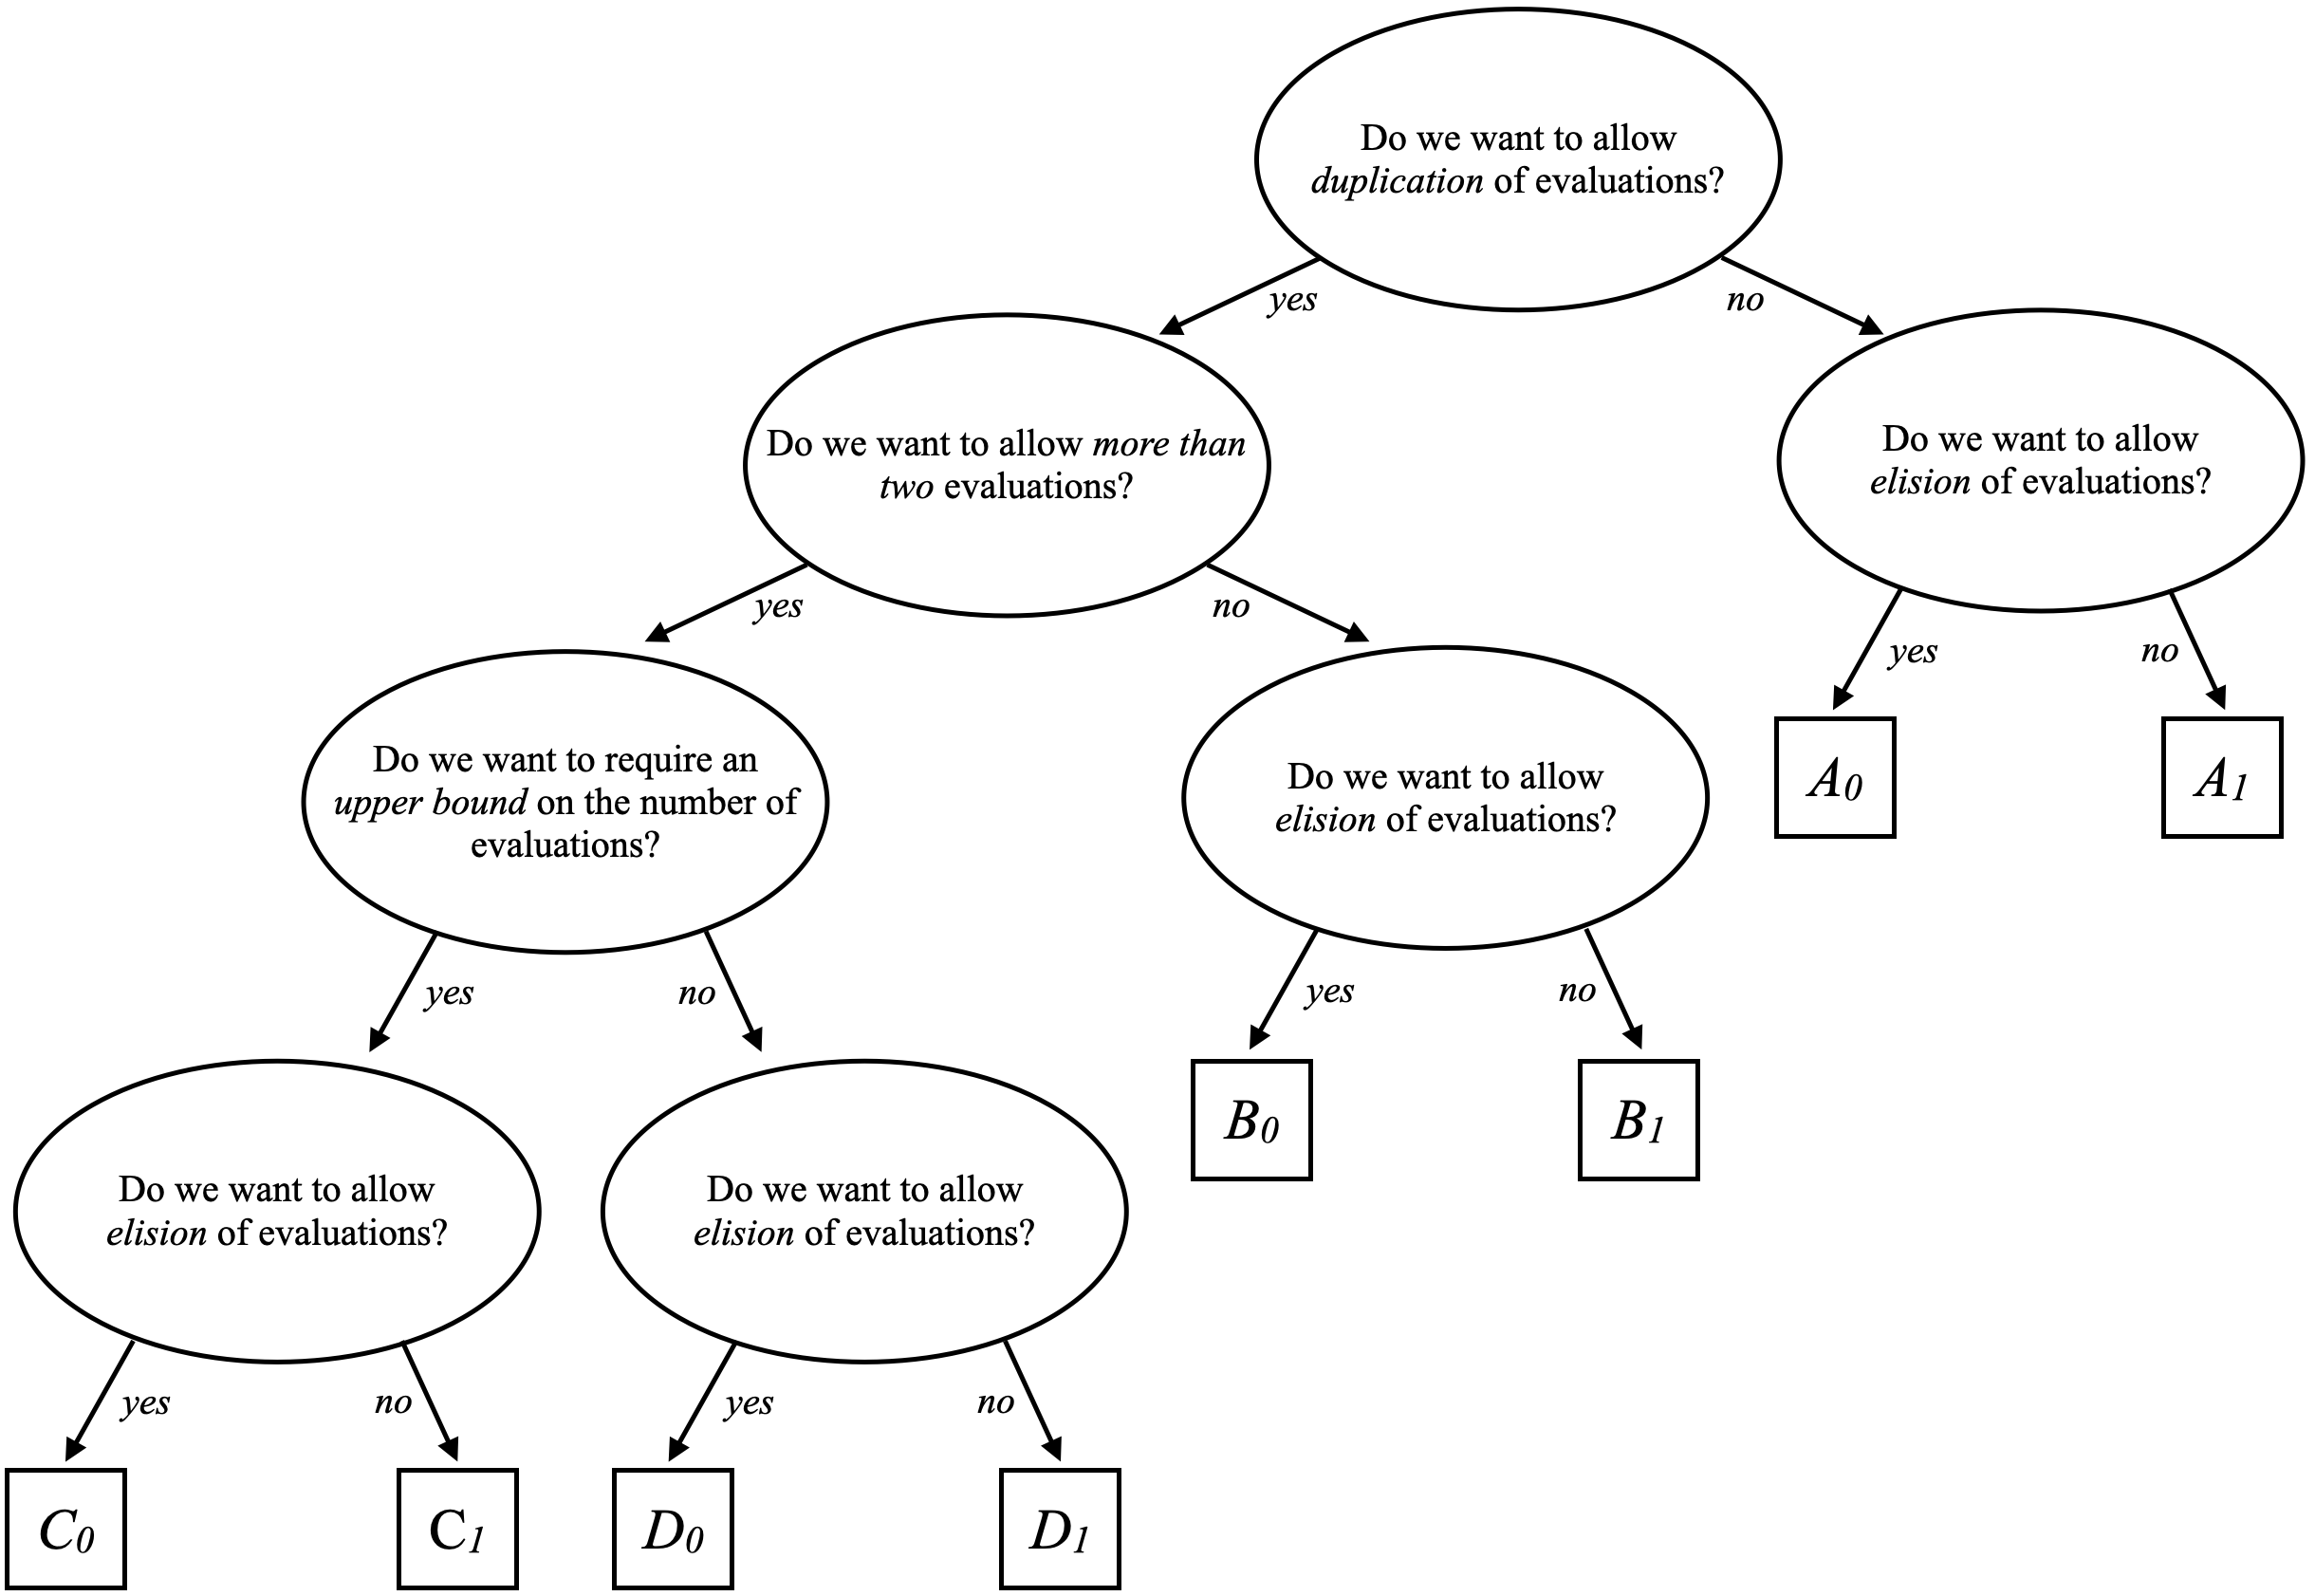
\includegraphics[width=1\linewidth]{images/p3228_fig1.png}
  \vspace{2mm}
  \caption{Possible decision tree for picking a solution.}
  \label{fig:prepost}
\end{figure}
%%%%%%%%%%%%%%%%%%%%%%%%%%%%%%%%%%%%%%%%%%%%%


\subsection{\tcode{contract_assert}}
For \tcode{contract_assert}, the decision matrix looks slightly differently. The need to support caller-/callee-side checking compatibility, which is the motivation for requirement 4, does not exist for \tcode{contract_assert}, because assertion statements can only appear inside the function body and are therefore always checked callee-side. Instead, there is a new requirement: it might be desirable to pick the same solution for \tcode{contract_assert} as we did for \tcode{pre} and \tcode{post} so that the three assertion kinds provided in the Contracts MVP behave in a consistent fashion.

Violating this consistency requirement would have implications for teachability, complexity of the language, etc. It would also widen the gap between the use of \tcode{pre} and the use of \tcode{contract_assert} at the start
of a function, or the use of \tcode{post} and the use of \tcode{contract_assert} before returning, which is the only mechanism offered by \cite{P2900R6} to insulate precondition and postcondition checks from client translation units when the developer considers them an implementation detail.

That said, the consistency requirement should be be weighed against the other requirements and we can in principle adopt a different solution for  \tcode{contract_assert} than for \tcode{pre} and \tcode{post}. For example, if we decide that requirement 1 (deterministic number of evaluations) is particularly important for \tcode{contract_assert}, because of the issue regarding existing practice with the \tcode{assert} macro discussed in Section~\ref{subsec:determ}, and that this is more important than the consistency requirement, or the requirements 5 --- 7 when applied to \tcode{contract_assert}, we could adopt solution $A_1$ for \tcode{contract_assert} despite having chosen a different solution for \tcode{pre} and \tcode{post}.



%%%%%%%%%%%%%%%%%%%%%%%%%%%%%%%%%%%%%%%%%%%%%
\footnotetext[1]{Note that the 0, 1, ``many'' requirement might be satisfiable for $B_0$ and $B_1$ if instead of generally allowing 2 evaluations, we specified these cases as \mbox{0 -- 1} evaluations on one or both sides of the call (caller-side and callee-side).}
%%%%%%%%%%%%%%%%%%%%%%%%%%%%%%%%%%%%%%%%%%%%%

\subsection{What are contract assertions?}

The current disagreement on the correct solution is  not only about which use cases and requirements to prioritise over others, but also about the correct mental model of what contract assertions \emph{are}.

One mental model is that the salient difference between contract assertions and existing control flow constructs such as \tcode{if} statements is that contract assertions can be ``turned off'' by choosing the \emph{ignore} evaluation semantic when compiling the program, similarly to how \tcode{assert} macros can be turned off by defining \tcode{NDEBUG}; apart from this ability, contract assertions are normal C++ code and contract predicates are normal C++ expressions. In this mental model, a \emph{checked} contract assertion such as \tcode{pre(expr)}, \tcode{post(expr)}, or \tcode{contract_assert(expr)} is effectively equivalent to:
\begin{codeblock}
if (!(expr))
  do_whatever_the_chosen_semantic_does();
\end{codeblock}

A different mental model is that contract assertions are not normal C++ code. Instead, they are \emph{annotations} that serve to inject additional information into the compiler about possible states that we consider to be incorrect. When choosing a \emph{checked} evaluation semantic, we instruct the compiler to use this information to identify such incorrect states, but we do not say how exactly the compiler is supposed to accomplish this: by evaluating \tcode{expr} or by using the information encoded in \tcode{expr} in some other way.

The first mental model leads to solution $A_1$; the second mental model leads to the other solutions, with $D_0$ being the most permissive about what the compiler is allowed to do with \tcode{expr} when checking for contract violations.

Notably, the current design in \cite{P2900R6} does not seem consistent in this regard. By choosing the ``natural syntax'' proposed in \cite{P2961R2} over the attribute-like syntax, we decided to make contract assertions look like normal code, rather than like annotations with special semantics, which is more consistent with the first mental model. Conversely, by allowing elision and duplication, we chose evaluation semantics that are more consistent with the second mental model.

%%%%%%%%%%%%%%%%%%%%%%%%%%%%%%%%%%%%%%%%%%%%%

%\pagebreak % MANUAL %%%%%%%%%
%\phantom{I really need a pagebreak here!}
%\pagebreak % MANUAL %%%%%%%%%

\section*{Acknowledgements}
Thanks to John Spicer, Ville Voutilainen, and Ga\v sper A\v zman for the illuminating discussions that led to this paper. Thanks to Jonas Persson, Andrew Tomazos, Joshua Berne, Jens Maurer, Andrzej Krzemie\' nski, and John Lakos for their helpful comments.


\renewcommand{\bibname}{References}
\bibliographystyle{abstract}
\bibliography{ref}

%%%%%%%%%%%%%%%%%%%%%%%%%%%%%%%%%%%%%%%%%%%%%

\end{document}
